\documentclass[letterpaper,10pt,oneside]{article} 
\usepackage[margin=2.54cm]{geometry}
\usepackage[spanish]{babel}
\newcommand\authormark[1]{\textsuperscript{#1}}
\usepackage[colorlinks=true,bookmarks=false,citecolor=black,urlcolor=black]{hyperref} 
\usepackage{times} 
\usepackage[table]{xcolor}
\usepackage{booktabs}
\usepackage{graphicx}
\usepackage{titlesec}
\usepackage{multicol}
\usepackage{float}

\titleformat{\section}
{\normalfont\fontsize{12pt}{14pt}\bfseries} % Fuente normal, tamaño 12pt, interlineado 14pt, en negrita
{\thesection}{1em}{} % Formato del número y separación

\begin{document}
	\begin{center}
		\fontsize{14}{16}\selectfont\bfseries
		Simulación de sistemas complejos mediante autómatas celulares neuronales
	\end{center}
	
	\begin{center}
		\fontsize{14}{16}\selectfont\bfseries
		\textit{Trabajo Terminal No. \_\_\_\_-\_\_\_}
	\end{center}
	
	\begin{center}
		\fontsize{12}{16}\selectfont
		\textit{Alumno: \authormark{*}Angeles López Erick Jesse\authormark{1}} \\
		\textit{Director: Juárez Martínez Genaro\authormark{1}} \\
		\textit{\authormark{*}e-mail: eangelesl1700@alumno.ipn.mx}
	\end{center}
	
	\textbf{Resumen} -- Este trabajo terminal tiene como objetivo desarrollar un sistema simulatario de espacios discretos bidimensionales para probar modelos de autómatas celulares neuronales. Se busca reemplazar las reglas fijas de los autómatas celulares tradicionales por redes neuronales, lo que permite que el sistema se adapte dinámicamente y mejore la generación, persistencia, recuperación y propagación de información. \\
	
	\textbf{Palabras clave} -- Autómatas celulares neuronales, Red neuronal, Sistemas complejos, Simulación
	
	\section{Introducción}
	
	La simulación de sistemas complejos ha emergido como una herramienta indispensable para la comprensión y el análisis de fenómenos en diversas áreas del conocimiento, desde la física y la biología hasta las ciencias sociales y económicas. Tradicionalmente, los autómatas celulares han servido como un modelo matemático fundamental para estudiar estos sistemas mediante la representación de procesos dinámicos. \\
	
	Los autómatas celulares son un modelo matemático que se componen de un espacio de celdas conectadas en un espacio discreto; en donde cada celda adquiere un estado que se actualiza en pasos constantes de tiempo con base en los estados de las celdas vecinas. Adicionalmente, se requiere de una función de transición que define como las celdas evolucionan de forma simultanea \cite{wolframCA, ZenilMartinez2024}. \\
	
	Entre los ejemplos clásicos se encuentra el \textit{Juego de la vida} de John Conway o los 256 autómatas celulares elementales estudiados por Stephen Wolfram. Estas herramientas han sido aplicadas en múltiples contextos como la simulación de incendios, modelización de distribuciones poblacionales, simulación de partículas y el análisis de ciclos climáticos \cite{darg}. No obstante, una limitación crítica de los modelos convencionales reside en la rigidez de sus funciones de transición, las cuales deben definirse de manera estática y anticipada, restringiendo la posibilidad de adaptarse a condiciones imprevistas o cambios en el entorno. Esta limitación motiva la búsqueda de nuevas metodologías capaces de incorporar mayor flexibilidad y adaptabilidad en la simulación de sistemas dinámicos. \\
	
	En este contexto, se busca la integración de redes neuronales en el marco de los autómatas celulares. Las redes neuronales, inspiradas en el funcionamiento del cerebro y su capacidad de aprendizaje, ofrecen la posibilidad de redefinir las reglas de transición de forma dinámica. Esto permite que el autómata celular se ajuste de manera autónoma a partir de la experiencia y el entrenamiento \cite{RN}. \\
	
	El presente proyecto de investigación propone superar las limitaciones de los autómatas celulares mediante la integración de redes neuronales en la definición de las reglas de transición, dando origen a los \textit{autómatas celulares neuronales}. En este enfoque, las reglas de actualización dejan de ser fijas y adquieren la capacidad de aprender y adaptarse a partir de los datos, lo que permite que el sistema se ajuste de forma dinámica ante comportamientos complejos y entornos variables \cite{redesNeuronales, distill}. Esta aproximación no solo busca ampliar el campo de aplicación de los autómatas celulares, sino que también busca abrir nuevas oportunidades para modelar y simular fenómenos de formas realistas.  \\
	
	Dadas las infinitas configuraciones de autómatas celulares, este proyecto se limita a un espacio bidimensional finito (con condiciones de frontera) y un conjunto finito y numerable de estados. Se buscan probar vecindades de Moore, Newman, entre otras, a expensas de la calidad requerida del modelo.
	
	\section{Objetivo}
	
	Desarrollar un sistema de simulación basado en los autómatas celulares neuronales en dos dimensiones, para analizar como se generan, mantienen, recuperan y propagan patrones de información en entornos complejos y dinámicos.
	
	\subsection{Objetivos específicos}
	
	\begin{itemize}
		\item Diseñar e implementar un simulador de espacios discretos bidimensionales que sirva de plataforma para estudiar los autómatas celulares neuronales.
		\item Entrenar y evaluar el desempeño de los autómatas celulares neuronales.
		\item Analizar y comparar diferentes comportamientos con base en la red neuronal establecida.
	\end{itemize}
	
	\section{Justificación}
	
	El presente proyecto de investigación surge ante la necesidad de superar las limitaciones inherentes a los modelos tradicionales de autómatas celulares, los cuales se caracterizan por depender de reglas de transición fijas y predeterminadas. Este enfoque restrictivo, si bien ha sido útil para modelar ciertos fenómenos, no permite capturar de forma adecuada la complejidad y la adaptabilidad de sistemas dinámicos presentes en entornos naturales, sociales y tecnológicos. Aunque es fortuito conocer el problema que resuelven algunos de los autómatas celulares mas conocidos, la definición matemática permite definir una infinidad de autómatas celulares sin objetivo aparente. \\
	
	Por esto, se propone la integración de redes neuronales en la definición de las reglas de transición, con el objetivo de desarrollar un modelo de \textit{autómata celular neuronal} capaz de aprender y adaptarse de manera autónoma a cambios en el entorno. Esto no solo amplía el alcance y la aplicabilidad de los autómatas celulares, sino que también abre un novedoso campo de estudio en el que se combinan herramientas de inteligencia artificial y simulación de sistemas complejos. \\
	
	La principal innovación de este enfoque reside en reemplazar las funciones de transición estáticas por modelos ajustables. Mediante técnicas de aprendizaje automático, la función de transición puede entrenarse con datos representativos, permitiendo que el sistema se adapte de manera autónoma a los cambios en el entorno \cite{pre}. \\
	
	Adicionalmente, este proyecto permitirá profundizar en técnicas de simulación, modelado matemático y redes neuronales, integrando conocimientos de ciencias de la computación, vida artificial y matemáticas. \\
	
	La experiencia adquirida durante el desarrollo e implementación de estos modelos abrirá puertas a futuras investigaciones y proyectos en el campo de la inteligencia artificial. Ademas, la creación de un entorno de código abierto contribuirá al avance del estado del arte y facilitará que otros investigadores puedan extender y aplicar estos conceptos.
	
	\section{Resultados Esperados}
	
	Como resultado de este trabajo terminal se espera obtener:
	\begin{itemize}
		\item \textbf{Aplicación de simulación desarrollada en Wolfram Mathematica y Python:}  
		Se creará una herramienta que permita visualizar, interactuar y exportar la evolución de los autómatas celulares neuronales de la cuadricula. Esta aplicación tendrá interfaz gráfica, módulo de entrenamiento y ejemplos prácticos, junto con el código fuente documentado para facilitar su replicación y extensión. Se propone la arquitectura de la figura \ref{fig:arquitectura} para el simulador. 
		
		\begin{figure}[H]
			\centering
			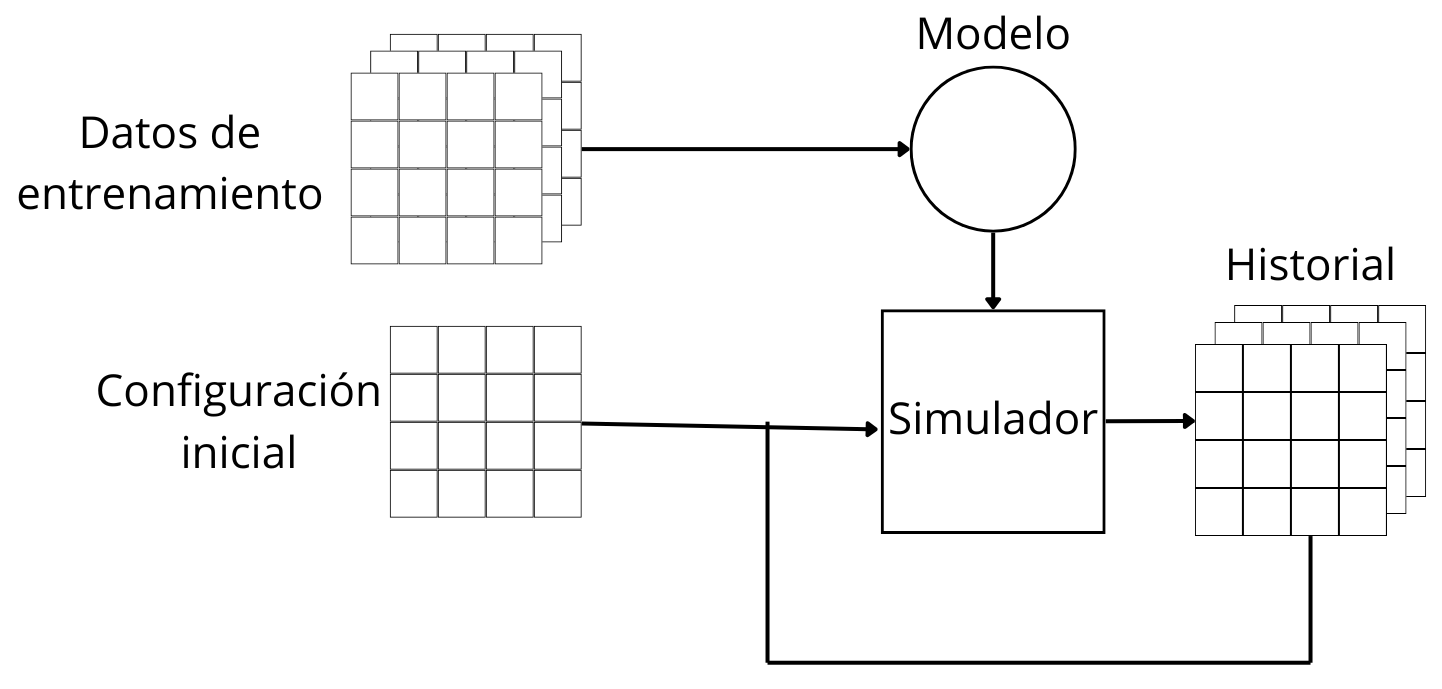
\includegraphics[width=0.85\textwidth]{img/arquitectura.png}
			\caption{Propuesta de arquitectura (Simulador)}
			\label{fig:arquitectura}
		\end{figure}
		
		\item \textbf{Documentación Técnica del Sistema:}  
		Se elaborará una documentación completa que incluya:
		\begin{itemize}
			\item Detalles de la implementación de los autómatas y la integración de las redes neuronales.
			\item Procedimientos de entrenamiento, métodos de validación y métricas de desempeño.
			\item Guías de instalación y uso de las aplicaciones.
		\end{itemize}
		\item \textbf{Artículo Académico:}  
		Se redactará un artículo en el que se describa la implementación de los autómatas celulares neuronales, abarcando:
		\begin{itemize}
			\item La metodología de integración de redes neuronales en la función de transición.
			\item Algoritmos, arquitecturas y técnicas de entrenamiento utilizadas.
			\item Un análisis comparativo con métodos tradicionales, comparando la adaptabilidad, robustez y eficiencia.
			\item Resultados experimentales, visualizaciones y discusión sobre la capacidad del modelo para reproducir patrones complejos.
		\end{itemize}
	\end{itemize}
	
	\section{Metodología}
	
	Para desarrollar este proyecto se seguirá un enfoque iterativo e incremental, que permite avanzar paso a paso y ajustar el modelo según se vayan obteniendo resultados. La metodología se divide en las siguientes fases:
	
	\begin{enumerate}
		\item \textbf{Planificación y Revisión Bibliográfica:} \\
		Definir el protocolo de investigación, revisar la literatura sobre autómatas celulares y redes neuronales, y estudiar investigaciones previas que hayan integrado ambos enfoques.
		
		\item \textbf{Diseño del Modelo:} \\
		Establecer la estructura del espacio discreto bidimensional y definir la arquitectura del autómata. Diseñar la red neuronal que se utilizará para actualizar las reglas de transición, y definir meta parámetros clave como el vecindario, número de estados y número de iteraciones.
		
		\item \textbf{Implementación:} \\
		Desarrollar el simulador e integrar la red neuronal en el modelo del autómata y desarrollar módulos para la visualización y el análisis de resultados.
		
		\item \textbf{Entrenamiento y Validación:} \\
		Entrenar y comparar los resultados de diferentes automatas celulares neuronales. Realizar experimentos para evaluar la capacidad del modelo de generar, mantener y recuperar información.
		
		\item \textbf{Documentación y Difusión:} \\
		Elaborar la documentación técnica y el manual de usuario del sistema. Además, se compartirá el código como proyecto de código abierto para facilitar futuras investigaciones.
	\end{enumerate}
	
	\section{Cronograma}
	
	\resizebox{\linewidth}{!}{%
		\begin{tabular}{p{5cm}*{10}{>{\centering\arraybackslash}p{1cm}}}
			\toprule
			\textbf{Actividad} & \textbf{AGO} & \textbf{SEP} & \textbf{OCT} & \textbf{NOV} & \textbf{DIC} & \textbf{ENE} & \textbf{FEB} & \textbf{MAR} & \textbf{ABR} & \textbf{MAY} \\
			\midrule
			\multicolumn{11}{l}{\textbf{Fase 1: Planificación y Revisión Bibliográfica}} \\
			Definir el protocolo y objetivos  & \cellcolor{gray!30} & \cellcolor{gray!30} &  &  &  &  &  &  &  &   \\
			
			Revisión del estado del arte       & \cellcolor{gray!30} & \cellcolor{gray!30} & \cellcolor{gray!30} &  &  &  &  &  &  &   \\
			
			Definir metodología y marco teórico  &  & \cellcolor{gray!30} & \cellcolor{gray!30} &  &  &  &  &  &  &   \\
			
			\midrule
			
			\multicolumn{11}{l}{\textbf{Fase 2: Diseño y Desarrollo del Simulador}} \\
			Diseño de la arquitectura del simulador &  &  & \cellcolor{gray!30} & \cellcolor{gray!30} &  &  &  &  &  &   \\
			
			Desarrollo del simulador  &  &  &  & \cellcolor{gray!30} & \cellcolor{gray!30} &  &  &  &  &   \\
			
			Integración de autómatas celulares   &  &  &  &  & \cellcolor{gray!30} & \cellcolor{gray!30} &  &  &  &   \\
			
			\midrule
			
			\multicolumn{11}{l}{\textbf{Fase 3: Entrenamiento y Validación de redes}} \\
			Entrenamiento y ajuste de la red  &  &  &  &  &  & \cellcolor{gray!30} & \cellcolor{gray!30} &  &  &   \\
			
			Experimentación y análisis de resultados  &  &  &  &  &  & \cellcolor{gray!30}  & \cellcolor{gray!30} & \cellcolor{gray!30} & \cellcolor{gray!30} &   \\
			
			Análisis de resultados  &  &  &  &  &  & \cellcolor{gray!30} & \cellcolor{gray!30} & \cellcolor{gray!30} & \cellcolor{gray!30} &   \\
			
			\midrule
			
			\multicolumn{11}{l}{\textbf{Fase 4: Documentación y Difusión}} \\
			Elaboración de la documentación técnica  &  &  &  &  &  &  &  & \cellcolor{gray!30}  & \cellcolor{gray!30} & \cellcolor{gray!30}  \\
			
			Redacción del artículo académico y presentación final  &  &  &  &  &  &  &  & \cellcolor{gray!30}  & \cellcolor{gray!30}  & \cellcolor{gray!30}  \\
			
			\bottomrule
		\end{tabular}
	}
	
	\section{Referencias} % crea sección numerada
	\renewcommand{\refname}{} % evita que el estilo ponga un título duplicado
	\bibliographystyle{IEEEtran}
	\bibliography{referencias}
	
	\section{Alumnos y directores}
	
\begin{tabular}{@{} p{0.45\textwidth} p{0.45\textwidth} @{}}
	\textit{Erick Jesse Angeles López}.- Alumno de la Carrera de Ingeniería en Inteligencia Artificial en la Escuela Superior de Cómputo, Boleta 2022630398, Tel. 5526641710, Email: eangelesl1700@alumno.ipn.mx
	&
	\textit{Genaro Juárez Martínez}.- Licenciado en Matemáticas Aplicadas y Computación egresado de la FES Acatlán, UNAM en 1998. Obtuvo el grado de Maestro en Ciencias de la Computación, asi como el de Doctorado en Ciencias de la computación en el CINVESTAV-IPN en 2001 y 2006 respectivamente. Actualmente se encuentra trabajando como profesor en la ESCOM del IPN. Áreas de interés: ciencias de la computación, computación no-convencional, vida artificial, robótica, sistemas complejos. Tel. 57296000 - Ext. 52067, Email: studentsresponsables@gmail.com
	
	 \\ & \\ & \\
	 & \\ & \\
	
	Firma:
	\rule{6cm}{0.4pt} & 
	
	Firma:
	\rule{6cm}{0.4pt} \\
	
	& \\ & \\
	& \\ & \\
	& \\ & \\
	& \\ & \\
	& \\ & \\
	& \\ & \\
	
	
	\cellcolor{gray!30} CARÁCTER: Confidencial & \\
	\cellcolor{gray!30} FUNDAMENTO LEGAL: Articulo 11 Fracc V y Artículos 108, 113, 117, de la Ley Federal de Transparencia y Acceso a la Información Pública. &\\
	\cellcolor{gray!30} PARTES CONFIDENCIALES: Número de boleta y teléfonos. & \\


\end{tabular}


\end{document}
